\subsection{Horus Gorgon}

\begin{center}
    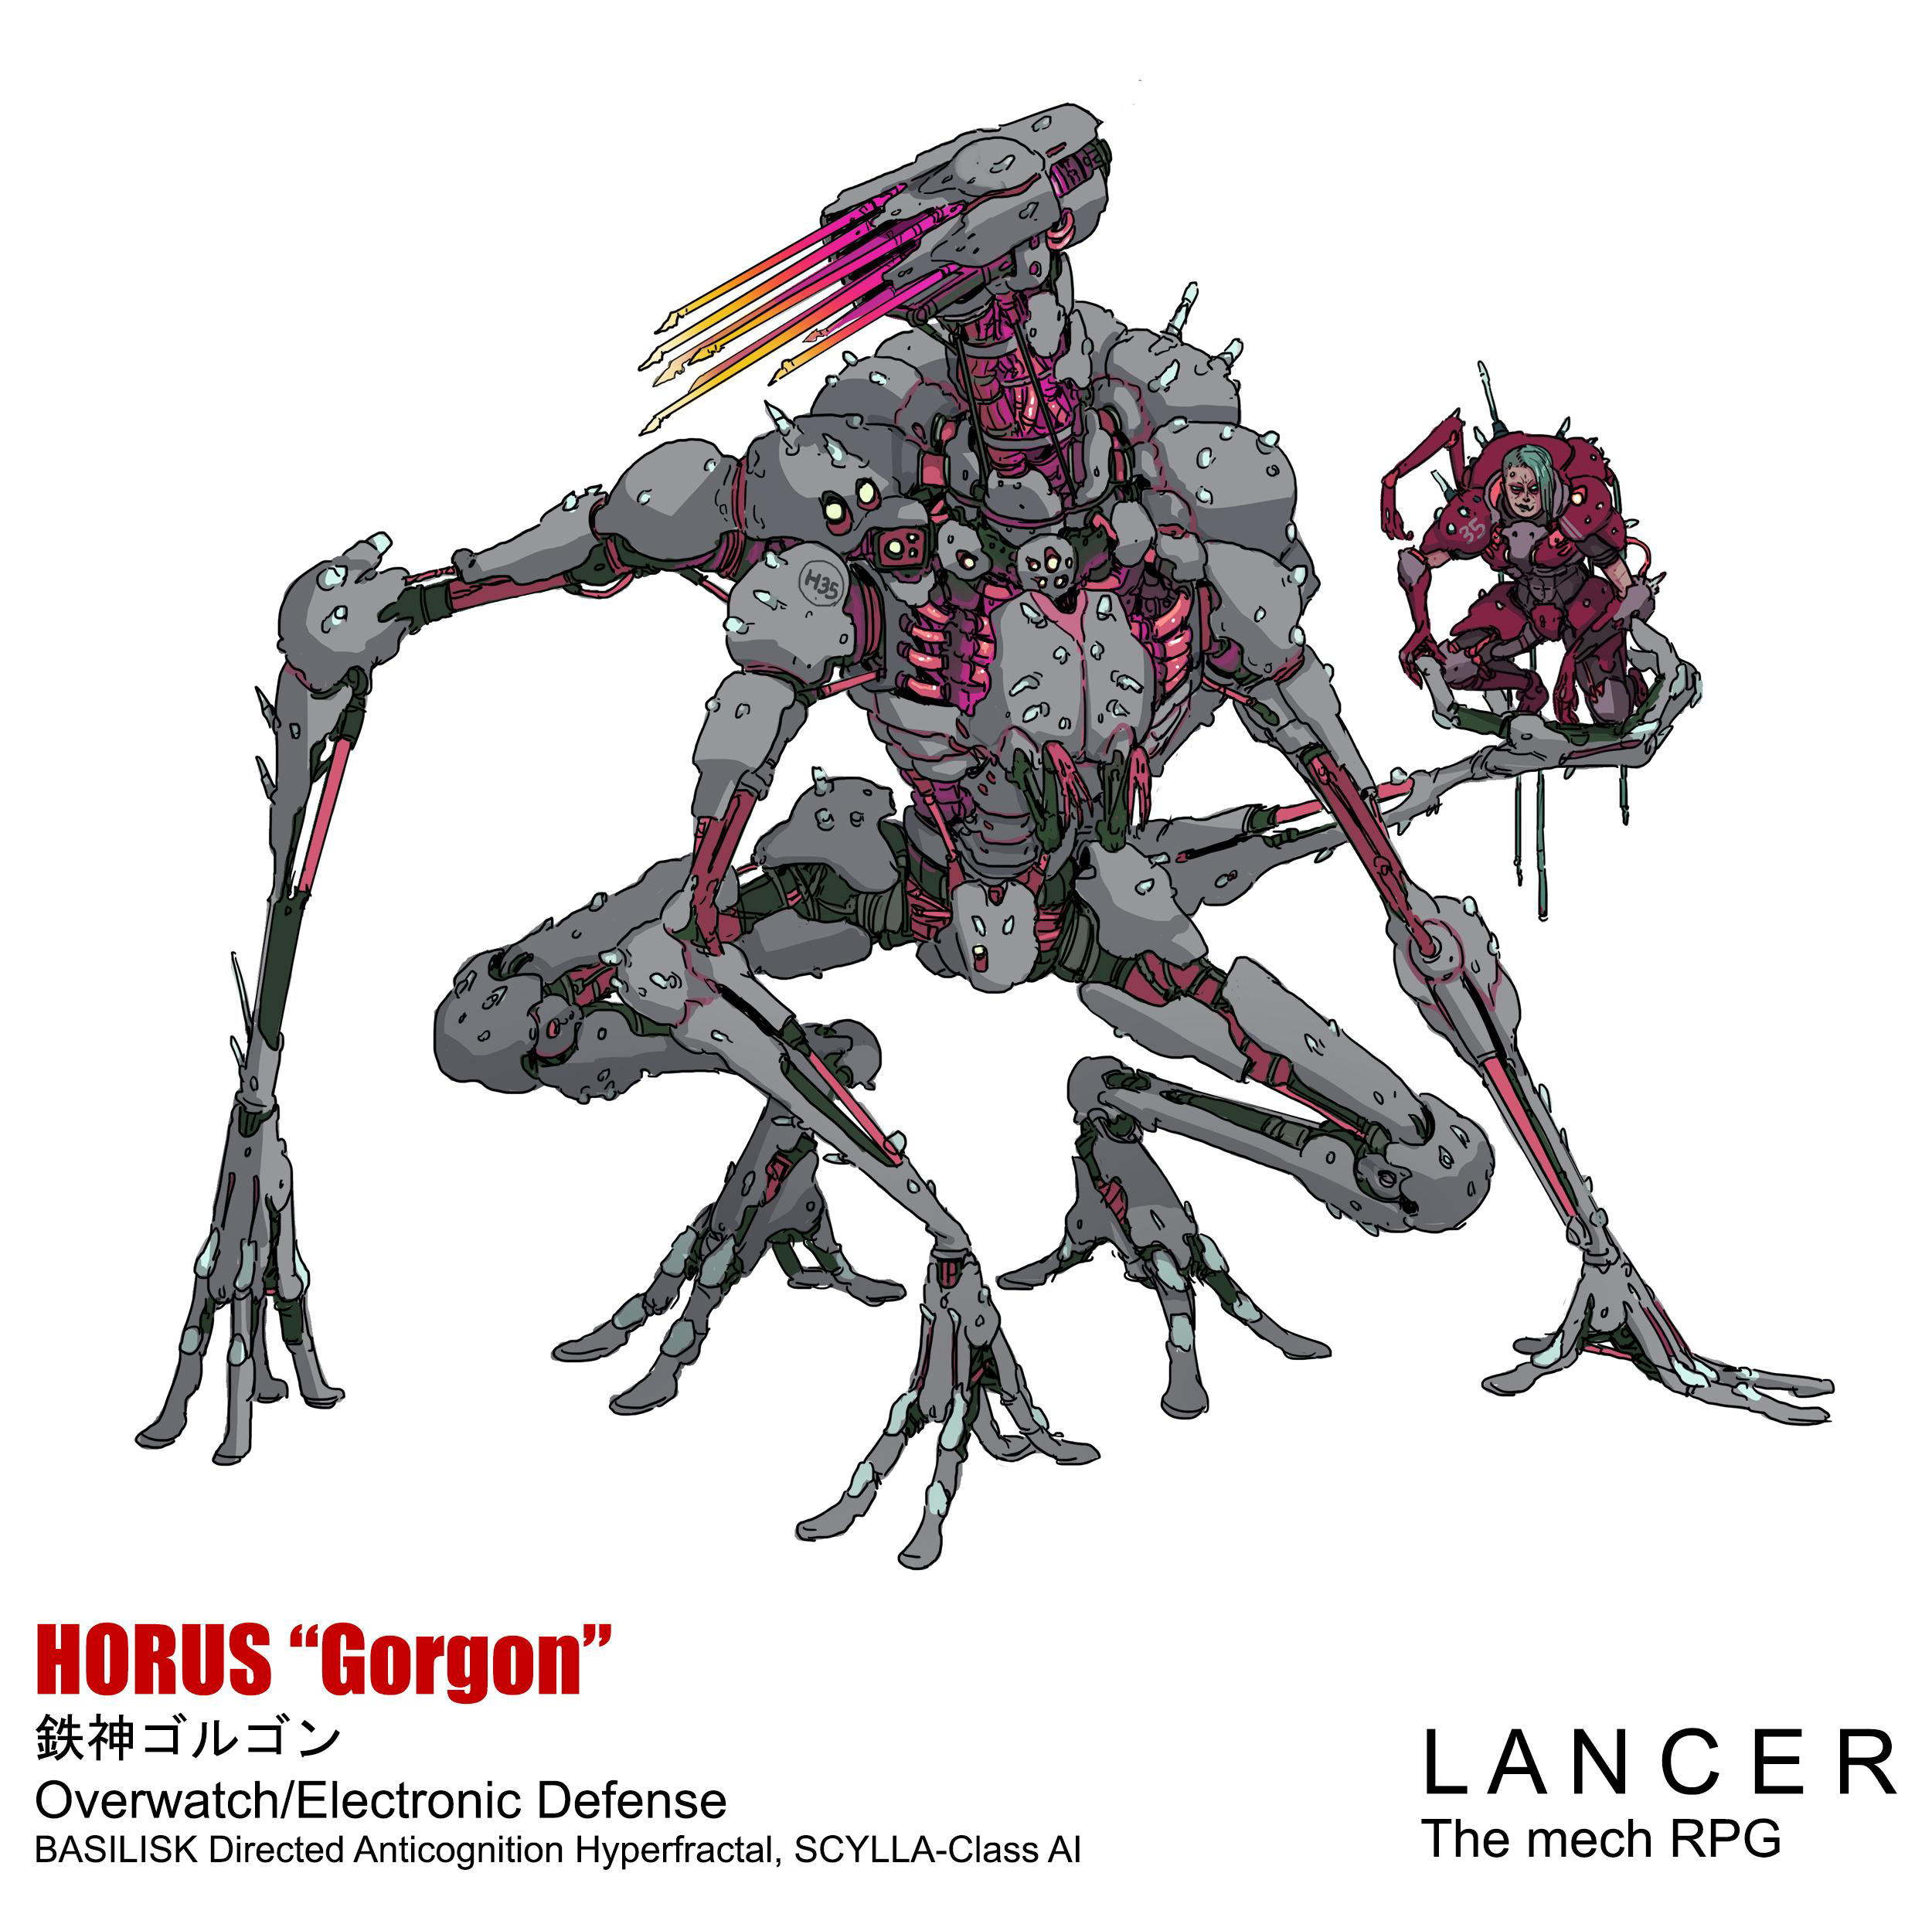
\includegraphics{Gorgon}
\end{center}

\begin{mech}{Horus}{Gorgon}

\fluff{The GORGON is unique among HORUS mech core parameters in that the classification describes a defensive rigging of weapons and systems meant to ensure personal and allied survival. The typical GORGON mounts multiple weapon systems meant to intercept and neutralize incoming fire and is widely feared for its ability to extrude a horrifying ‘basilisk’, a projected pattern of impossible visual data so toxic to logical thought that it causes massive failure in NHPs and can cause mild brain damage in humans.}

\begin{license}
\item Sentinel Drone Nexus, Point Defense Drone
\item GORGON FRAME,  //SCORPION v70.1, MONITOR Module
\item SCYLLA Class AI, Vorpal Gun
\end{license}


\frameBox
[hp = 10,
evasion = 8,
speed = 3,
heat cap = 6,
sensors = 10,
armor = 0,
e-defense = 12,
size = 2,
repair cap = 3,
tech attack = +1,
traits = {
     \textbf{Meta-state Paralysis}: Any attacker that rolls a 1 or 2 on their d20 roll to attack the Gorgon is automatically stunned until the end of their next turn (their attack also automatically misses).

     \textbf{Guardian}: Adjacent allies can use the GORGON for light cover
     },
sp = 6,
mount one = flex mount,
mount two = main mount,
mount three = main mount,
core system name = Harnessed Basilisk,
core system text = {The BASILISK Directed Anticognition Hyperfractal is a Horus-script-derived liturgical code translated for chassis-tier engagement. Typically point-broadcasted from a communications laser, the BASILISK liturgicode is a memetic weapon that affects any who can see it, unless they have had the proper tempering. Survivors often exhibit momentary paralysis, corporeal alienation, and consciousness destabilization. Anticognition Hyperfractals are classified as paracausal weapons -- as of yet, there is no effective defense against them.},
core active name = Extrude Basilisk,
core active text = {Quick Action

Your mech projects a horrifying Basilisk pattern, incredibly harmful to NHPs, software, and hard to look at even for humans (typically causes 3-5 hours of headaches and intense subdermal bleeding, can often cause blood vessels to pop in the eye). Until the end of the current combat, any target (mech, human, or biological) that attacks either you or any ally within range 5 of you must first pass a systems check or be stunned until the end of their next turn. A target can only be stunned once by this effect per combat.
}]


Sentinel Drone Nexus
Sentinel drones take the same principal of assassin drones but make their presence noticeable; as it is not necessary for them to be subtle, sentinel drones have the ability for autonomous movement, often engaging in a patrol doctrine dictated by their commander. Sentinel drones lock on to aggressive actions by enemy combatants and move quickly to shut them down.

2 SP
Drone, Quick Action
You fire this drone as a quick action at a free space in sensor range, creating a burst 2 area centered on the drone. It can be attacked and destroyed as normal. You can move the area the drone effects (and the drone itself) by taking this action again. While the drone is active, any hostile target that attacks in that area takes 1 kinetic damage before they attack as the drone shoots them (no check or attack roll required).

Point Defense Drone
PDWs are mainstays in stellar navies, used to engage with and destroy incoming missiles and torpedoes. On a mech core, PDWs adopt the same role and then some, engaging not only incoming ordnance (missiles, FRAMEs), but nearby hostile soft targets as well.

2 SP
Quick Action
You can fire this drone to any free space in sensor range, where it hovers in place and creates a burst 1 area centered on the drone. Attacks against yourself or allied actors in the area that deal explosive damage or have the nexus, smart, or launcher tags attack with +2 difficulty.

MONITOR Module
A MONITOR subroutine enhances stock targeting software’s IFF protocol to ensure constant coverage of allied mech cores, even when pilots are occupied in other necessary actions.

2 SP
Quick Action
When you take this quick action, choose an adjacent ally and roll a 1d3 to gain that many charges. Until the start of your next turn, when that ally is attacked by a hostile actor, you can spend a charge to attack that target if they are in range as a reaction, with +1 difficulty. You lose these charges at the start of your next turn.

//SCORPION v. 70.1
The //SCORPION program has a long and storied history in the Omninet. Originally constructed from fill code sourced from a research paper on AI hardcode reflex-response, //SCORPION evolved from a simple packet interpreter to an anti-incursion program. HORUS closely guards the full text of //SCORPION’s source code: they’re rumored to have installed a kill switch into the program, but the existence of such a switch has never been confirmed.

2 SP, Unique
If any hostile tech action or attack attempt on you or any adjacent ally fails or misses, you may choose one of the following results for the attacker:
The attacker is Impaired until the end of its next turn
The attacker is Jammed until the end of its next turn
The attacker takes 3 heat

Vorpal Gun
DO NOT STARE DIRECTLY INTO THE APERTURE.

Main Cannon
Range 5
2d6 kinetic damage
This weapon can’t be fired normally or used for reaction fire. Instead, it can only be fired 1/round as a reaction to any ally taking damage from an actor in its range.

SCYLLA Class AI
...first isolated GORGON strains hid a secret: SCYLLA, a dormant NHP unknown to Union until its first manifestation in 4852, when it woke after a control-fabricate GORGON was run through a USB Balwinder-Bolaño stress test.

SCYLLA proved difficult to manage, and USB ontologisticians were unable to pin down a stable subjectivity. SCYLLA reached cascade within minutes of emerging from dormancy; to prevent further metastatic cascade, the security forces present engaged the SCYLLA prime unit, defabricating it with a steady bombardment of kinetic and energy weapons...

[there, a little history, a little background. A little knowledge of where this little one came from. treat it with kindness, and it will love you as a loyal dog does its master]

3 SP, Unique
AI

Your mech gains the AI property and the Unleash SCYLLA action
Unleash SCYLLA
Quick Action
  	3 heat (self)
Until the start of your next turn, you gain 2 reactions. These reactions can be used to make a skirmish action as a reaction with +2 difficulty. You set the trigger for these reactions from the following list, and must attack the target that activates the trigger:
An enemy attacks you or an allied target within range 5 of you
An enemy attempts to interact with an object in the environment (not held, worn, or part of a mech) that you choose when you take this action


\end{mech}
